% ============================================================
%  HCI PROJECT REPORT — Tabla Restaurant Discovery Website
%  CS5015 — Human Computer Interaction
%  Compile: pdflatex hci_report.tex  (run twice for TOC)
% ============================================================
\documentclass[11pt,a4paper]{article}

\usepackage[margin=2cm]{geometry}
\usepackage{graphicx}
\usepackage[hidelinks,colorlinks=true,linkcolor=blue,urlcolor=blue]{hyperref}
\usepackage{enumitem}
\usepackage{fancyhdr}
\usepackage{booktabs}
\usepackage{array}
\usepackage{longtable}
\usepackage{xcolor}
\usepackage{titlesec}
\usepackage{caption}
\usepackage{float}
\usepackage{parskip}
\usepackage{setspace}
\usepackage{tabularx}
\usepackage{multirow}

\graphicspath{{pics/}}

\pagestyle{fancy}
\fancyhf{}
\rhead{CS5015 — HCI Project Report}
\lhead{Tabla: Restaurant Discovery Website}
\cfoot{\thepage}
\renewcommand{\headrulewidth}{0.4pt}

\setstretch{1.2}
\setlength{\parindent}{0pt}
\setlength{\parskip}{4pt}

\titleformat{\section}{\large\bfseries}{}{0em}{\thesection\quad}
\titleformat{\subsection}{\normalsize\bfseries}{}{0em}{\thesubsection\quad}
\titleformat{\subsubsection}{\small\bfseries}{}{0em}{}

\definecolor{lawblue}{RGB}{30,80,160}
\definecolor{fixgreen}{RGB}{20,120,60}
\definecolor{violred}{RGB}{180,30,30}

% ============================================================
\begin{document}
% ── Title Page ───────────────────────────────────────────────
\begin{titlepage}
  \centering\vspace*{1.5cm}
  {\Huge\bfseries Tabla: Restaurant Discovery Website\par}
  \vspace{0.4cm}{\large\itshape An HCI Design \& Evaluation Report\par}
  \vspace{1.5cm}\hrule\vspace{0.3cm}
  \begin{tabular}{rl}
    \textbf{Course:}     & CS5015 — Human Computer Interaction \\[3pt]
    \textbf{Instructor:} & Prof.\ B.\ Sivaselvan \\[3pt]
    \textbf{Student:}    & Sudarshan Sudhakar \\[3pt]
    \textbf{Roll No:}    & CS23B2007 \\[3pt]
    \textbf{Date:}       & February 2026 \\
  \end{tabular}
  \vspace{0.3cm}\hrule\vspace{1.5cm}
  \includegraphics[width=0.82\linewidth]{tabla/landing1.png}
  \captionof{figure}{Tabla — Cinematic Landing Page (Sequence 1)}
  \vfill{\small Submitted in partial fulfilment of the requirements of CS5015.\par}
\end{titlepage}

\tableofcontents\newpage

% ============================================================
\section{Website Overview}
% ============================================================

\subsection{Purpose and Target Users}
\textbf{Tabla} is a full-stack single-page restaurant discovery application for urban food enthusiasts in Chennai, Mumbai, and Bangalore. Three primary user types: \textbf{Casual Diners} (search by cuisine/location), \textbf{Fine-Dining Planners} (filter by rating, price, ambiance), and \textbf{Deal Hunters} (time-limited discounts).

\subsection{Core Features}
(1)~Cinematic frame-by-frame intro scroll (Seq.\ 1 \& 2) via canvas renderer. (2)~Smart restaurant grid with real-time search, multi-dimensional filters, lazy-loaded images. (3)~Three-step reservation modal (date/time, guest count, email confirmation). (4)~SPA navigation across six tabs: Explore, Near Me, Cuisines, Saved, Deals, Sign In. (5)~Keyboard shortcut overlay, skip intro, review modal, persistent favourites.

\subsection{UI Walkthrough}
\begin{figure}[H]\centering
  \begin{minipage}{0.49\linewidth}
    \includegraphics[width=\linewidth]{tabla/landing2.png}
    \caption{Cinematic Intro — Sequence 2}
  \end{minipage}\hfill
  \begin{minipage}{0.49\linewidth}
    \includegraphics[width=\linewidth]{tabla/landing3.png}
    \caption{Cinematic Intro — Sequence 3}
  \end{minipage}
\end{figure}

\begin{figure}[H]\centering
  \includegraphics[width=\linewidth]{tabla/main page.png}
  \caption{Main App — Hero Search \& Quick Filter Bar}
\end{figure}

\begin{figure}[H]\centering
  \begin{minipage}{0.49\linewidth}
    \includegraphics[width=\linewidth]{tabla/filters.png}
    \caption{Advanced Filter Drawer}
  \end{minipage}\hfill
  \begin{minipage}{0.49\linewidth}
    \includegraphics[width=\linewidth]{tabla/near me.png}
    \caption{Near Me Tab — Geo-sorted list}
  \end{minipage}
\end{figure}

\begin{figure}[H]\centering
  \begin{minipage}{0.49\linewidth}
    \includegraphics[width=\linewidth]{tabla/cusines.png}
    \caption{Cuisines Tab — Category cards}
  \end{minipage}\hfill
  \begin{minipage}{0.49\linewidth}
    \includegraphics[width=\linewidth]{tabla/deals.png}
    \caption{Deals Tab — Countdown timers}
  \end{minipage}
\end{figure}

\begin{figure}[H]\centering
  \includegraphics[width=0.6\linewidth]{tabla/saved.png}
  \caption{Saved Tab — Favourited restaurants}
\end{figure}

\begin{figure}[H]\centering
  \begin{minipage}{0.32\linewidth}
    \includegraphics[width=\linewidth]{tabla/reservation1.png}
    \caption{Reservation Step 1}
  \end{minipage}\hfill
  \begin{minipage}{0.32\linewidth}
    \includegraphics[width=\linewidth]{tabla/reservation2.png}
    \caption{Reservation Step 2}
  \end{minipage}\hfill
  \begin{minipage}{0.32\linewidth}
    \includegraphics[width=\linewidth]{tabla/reservation3.png}
    \caption{Reservation Step 3}
  \end{minipage}
\end{figure}

\begin{figure}[H]\centering
  \begin{minipage}{0.32\linewidth}
    \includegraphics[width=\linewidth]{tabla/review1.png}
    \caption{Review Modal Step 1}
  \end{minipage}\hfill
  \begin{minipage}{0.32\linewidth}
    \includegraphics[width=\linewidth]{tabla/review2.png}
    \caption{Review Modal Step 2}
  \end{minipage}\hfill
  \begin{minipage}{0.32\linewidth}
    \includegraphics[width=\linewidth]{tabla/review3.png}
    \caption{Review Modal Success}
  \end{minipage}
\end{figure}

\begin{figure}[H]\centering
  \begin{minipage}{0.45\linewidth}
    \includegraphics[width=\linewidth]{tabla/shortcuts.png}
    \caption{Keyboard Shortcut Overlay}
  \end{minipage}\hfill
  \begin{minipage}{0.45\linewidth}
    \begin{minipage}{\linewidth}
      \includegraphics[width=\linewidth]{tabla/fav(heart).png}
      \caption{Heart/Favourite Toggle}
    \end{minipage}\\[6pt]
    \begin{minipage}{\linewidth}
      \includegraphics[width=\linewidth]{tabla/skip intro icon.png}
      \caption{Skip Intro Button}
    \end{minipage}
  \end{minipage}
\end{figure}

% ============================================================
\newpage
\section{Yelp HCI Violations — and How Tabla Fixes Them}
% ============================================================

\noindent This section presents five HCI design-law violations observed on Yelp (early 2026), each paired with how Tabla addresses the same concern.

% ── Violation 1 ──────────────────────────────────────────────
\subsection{\textcolor{violred}{V1 — Hick's Law: Choice Overload} \hfill\textcolor{fixgreen}{Fix: Single-Focus Hero}}

\textbf{Law (Lec~07, p.8--9):} Decision time $\propto \log_2(n+1)$ choices. More options = more delay.

\textbf{Yelp's Violation:} The landing page simultaneously displays 20+ category icons, two search bars, promotional banners, and editorial carousels. Users are overwhelmed before forming intent (see Fig.~\ref{fig:yelp-landing}).

\begin{figure}[H]\centering
  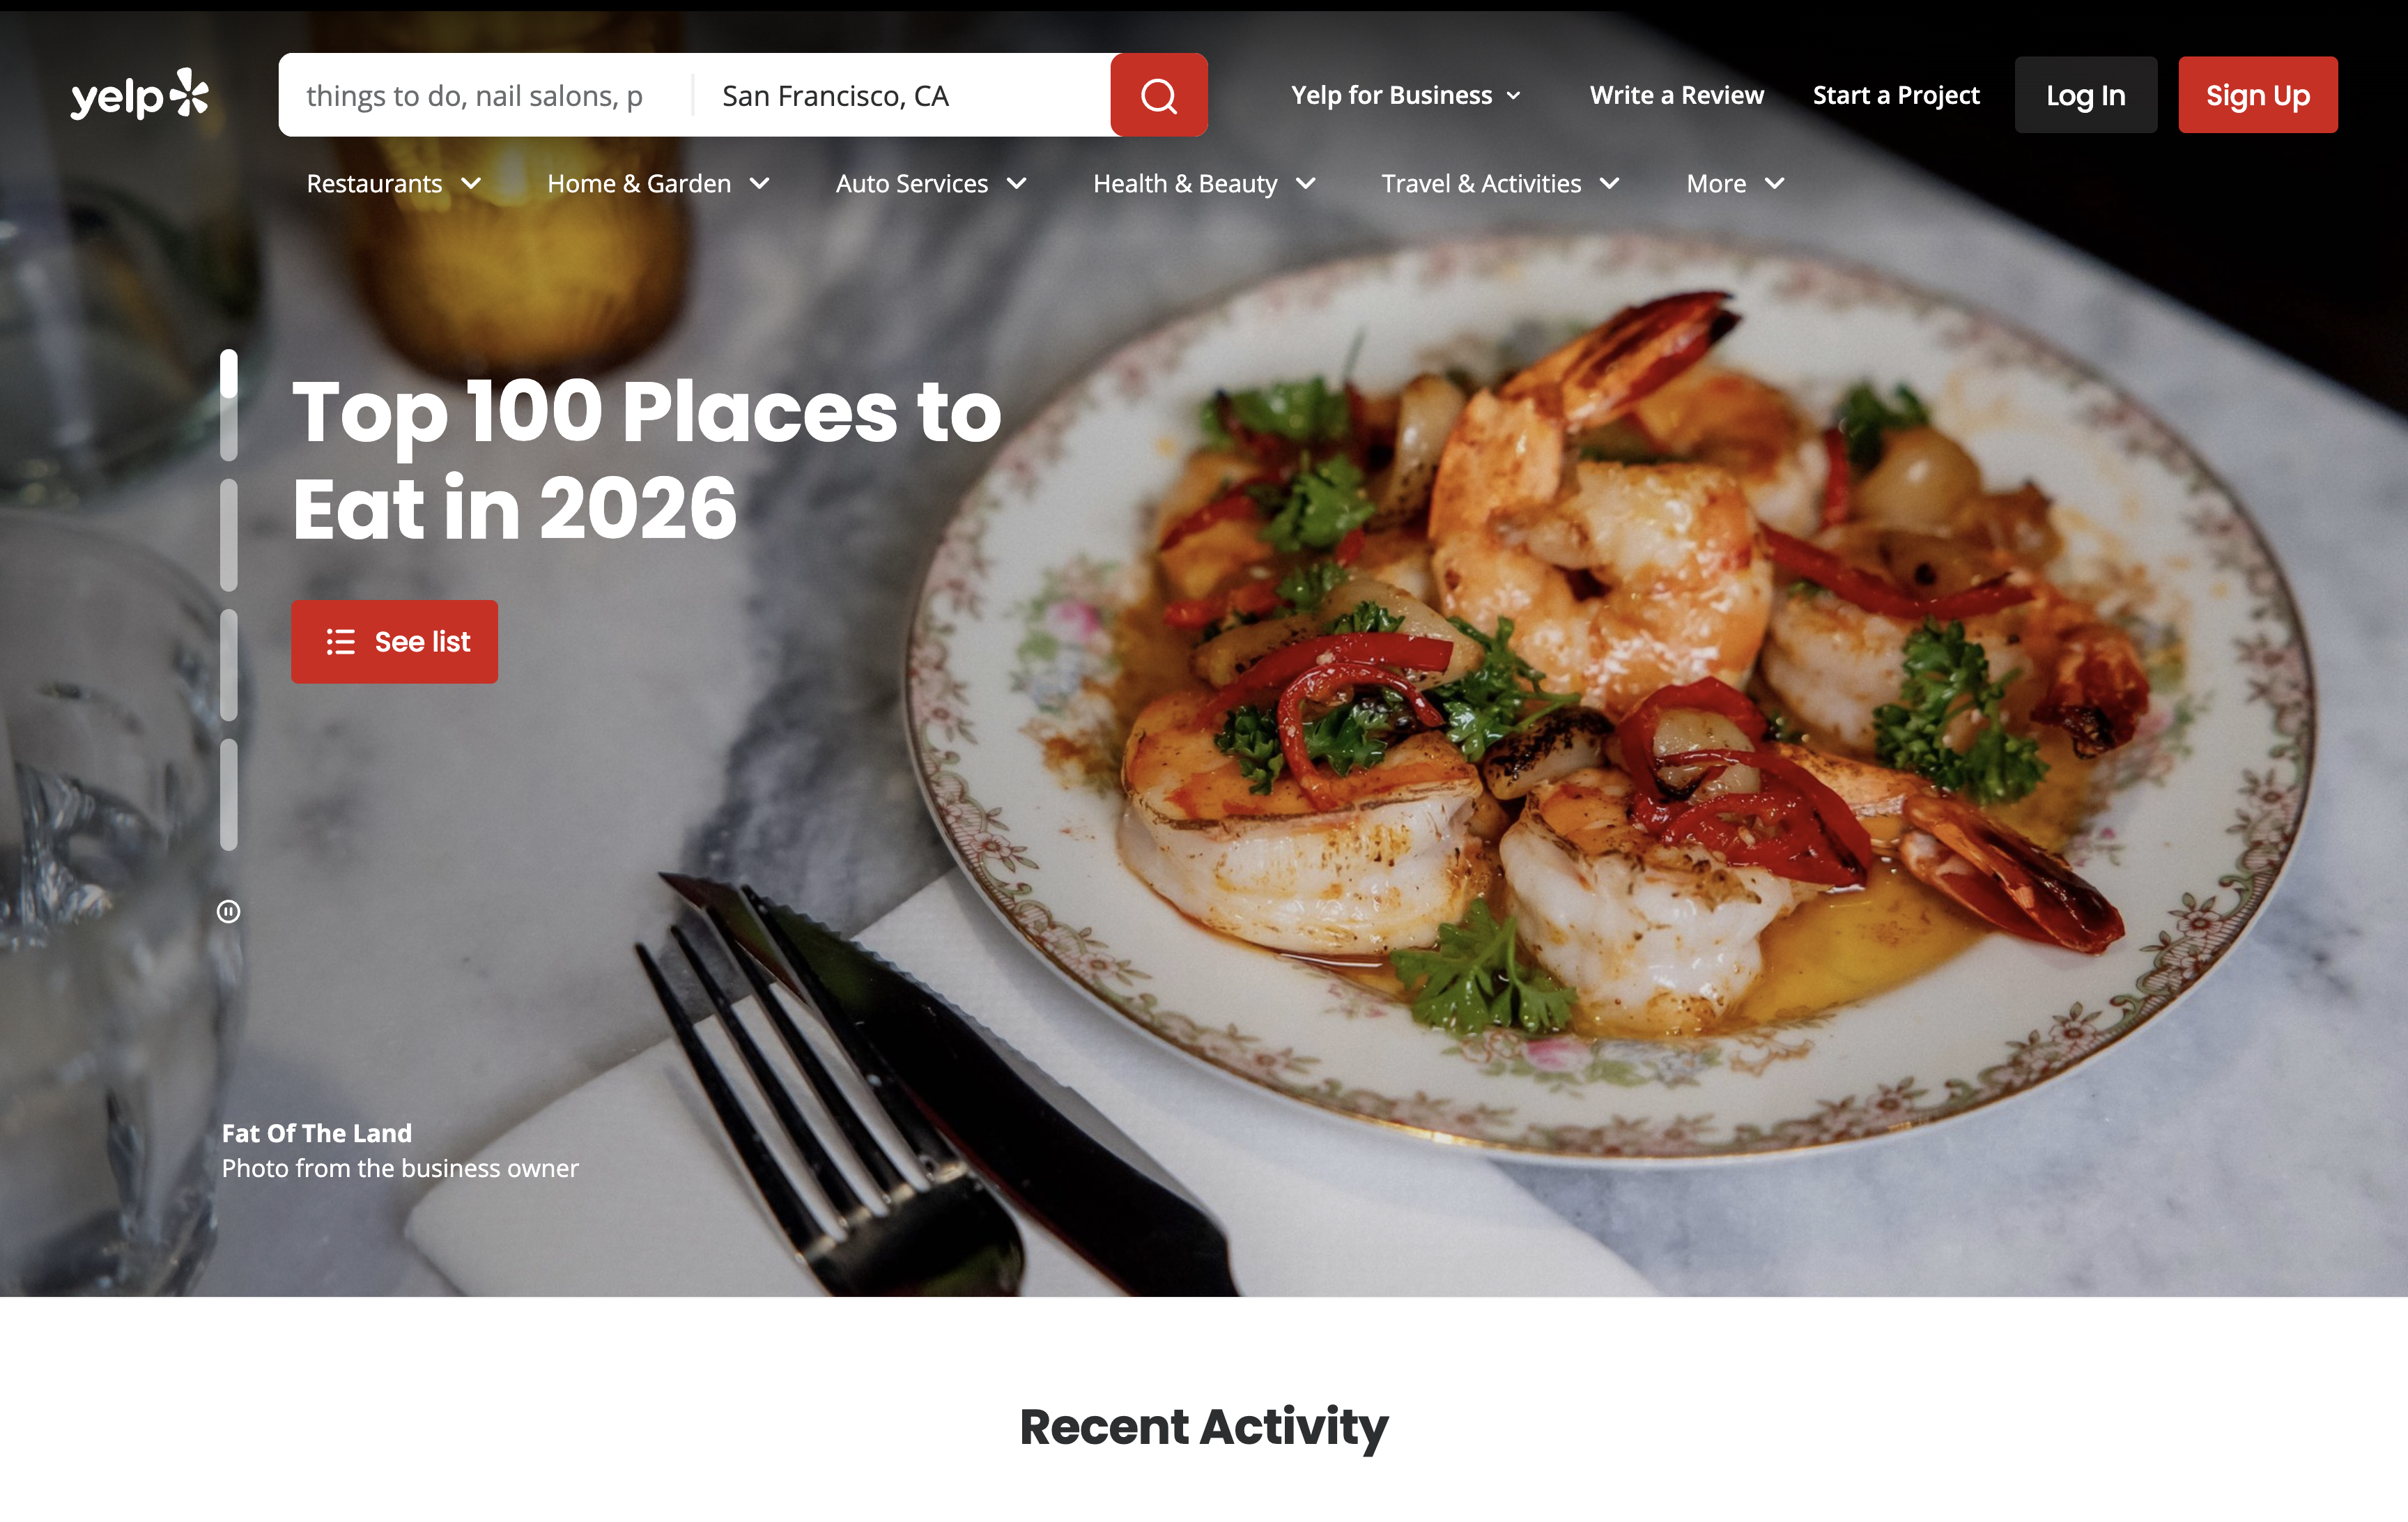
\includegraphics[width=0.9\linewidth]{yelp/landing page.png}
  \caption{Yelp Landing — Information overload violating Hick's Law}
  \label{fig:yelp-landing}
\end{figure}

\textcolor{fixgreen}{\textbf{Tabla Fix:}} A single full-screen hero presents exactly \emph{one} action (search bar). Secondary cuisine chips are limited to five (within the 7$\pm$2 rule). Progressive-disclosure hides advanced filters behind ``More Filters~$\downarrow$''. This also satisfies \textbf{Nielsen H8 — Aesthetic \& Minimalist Design} (Lec~03, p.8).

% ── Violation 2 ──────────────────────────────────────────────
\subsection{\textcolor{violred}{V2 — Fitts's Law: Tiny Action Buttons} \hfill\textcolor{fixgreen}{Fix: 44px Targets}}

\textbf{Law (Lec~07, p.4--7):} $MT = a + b\log_2(2A/W)$. Larger, closer targets are faster to acquire.

\textbf{Yelp's Violation:} ``Write a Review'', ``Add Photo'', and ``Save'' are sub-16\,px icon-only buttons in a narrow row, far from the content column — especially problematic on mobile (Fig.~\ref{fig:yelp-detail}).

\begin{figure}[H]\centering
  \includegraphics[width=0.9\linewidth]{yelp/rest page.png}
  \caption{Yelp Restaurant Detail — Small buttons violating Fitts's Law}
  \label{fig:yelp-detail}
\end{figure}

\textcolor{fixgreen}{\textbf{Tabla Fix:}} Reserve, Review, and Directions buttons span full card width at $\geq$44\,px height. The primary ``Find'' button is placed directly adjacent to the search input (zero extra travel). Destructive actions (clear filters) are intentionally small per Fitts's inverse.

% ── Violation 3 ──────────────────────────────────────────────
\subsection{\textcolor{violred}{V3 — Jakob's Law: Non-Standard Navigation} \hfill\textcolor{fixgreen}{Fix: Industry Conventions}}

\textbf{Law (Lec~02, p.9; Lec~08, p.7--8):} Users import mental models from other sites — they prefer what they already know.

\textbf{Yelp's Violation:} Profile, notifications, and saved collections are buried inside a hamburger menu; slug-based URLs break browser back-navigation (Fig.~\ref{fig:yelp-restpage}).

\begin{figure}[H]\centering
  \includegraphics[width=0.9\linewidth]{yelp/rest page 2.png}
  \caption{Yelp Restaurant Page — Unconventional layout violating Jakob's Law}
  \label{fig:yelp-restpage}
\end{figure}

\textcolor{fixgreen}{\textbf{Tabla Fix:}} Sticky top-nav mirrors Zomato/Swiggy/Google Maps. Heart icon (Instagram/Airbnb convention), star ratings, price symbols (₹/₹₹/₹₹₹), and a three-step reservation flow (OpenTable convention) all leverage existing mental models.

% ── Violation 4 ──────────────────────────────────────────────
\subsection{\textcolor{violred}{V4 — Miller's Law: 30+ Uncategorised Filters} \hfill\textcolor{fixgreen}{Fix: Chunked Groups}}

\textbf{Law (Lec~07, p.1):} STM holds $7\pm2$ chunks; Primacy \& Recency effect (Lec~07, p.2--3) causes middle-option blindness.

\textbf{Yelp's Violation:} 30+ cuisine/ambiance checkboxes in one flat scrollable list with no grouping (Fig.~\ref{fig:yelp-grid}).

\begin{figure}[H]\centering
  \includegraphics[width=0.9\linewidth]{yelp/restaurant grid.png}
  \caption{Yelp Grid — Excessive uncategorised filters violating Miller's Law}
  \label{fig:yelp-grid}
\end{figure}

\textcolor{fixgreen}{\textbf{Tabla Fix:}} Filters are chunked into four logical groups: Quick (4 chips), Price (3 tiers), Cuisine (6 cards), Advanced (drawer). Each group stays within $7\pm2$. Restaurant cards show exactly 6 fields; filter tags are capped at 3 per card.

% ── Violation 5 ──────────────────────────────────────────────
\subsection{\textcolor{violred}{V5 — Nielsen H1 \& Norman Feedback: Silent Confirmations} \hfill\textcolor{fixgreen}{Fix: Persistent Status}}

\textbf{Law (Lec~03, p.6, p.9):} The system must always keep users informed; Shneiderman Rule: ``Offer Informative Feedback'' and ``Design Dialogs for Closure'' (Lec~03, p.2).

\textbf{Yelp's Violation:} Review submission shows a 2-second text banner then vanishes. Photo upload progress shows only a spinner — no percentage. No persisted ``submitted'' state (Fig.~\ref{fig:yelp-rest2}).

\begin{figure}[H]\centering
  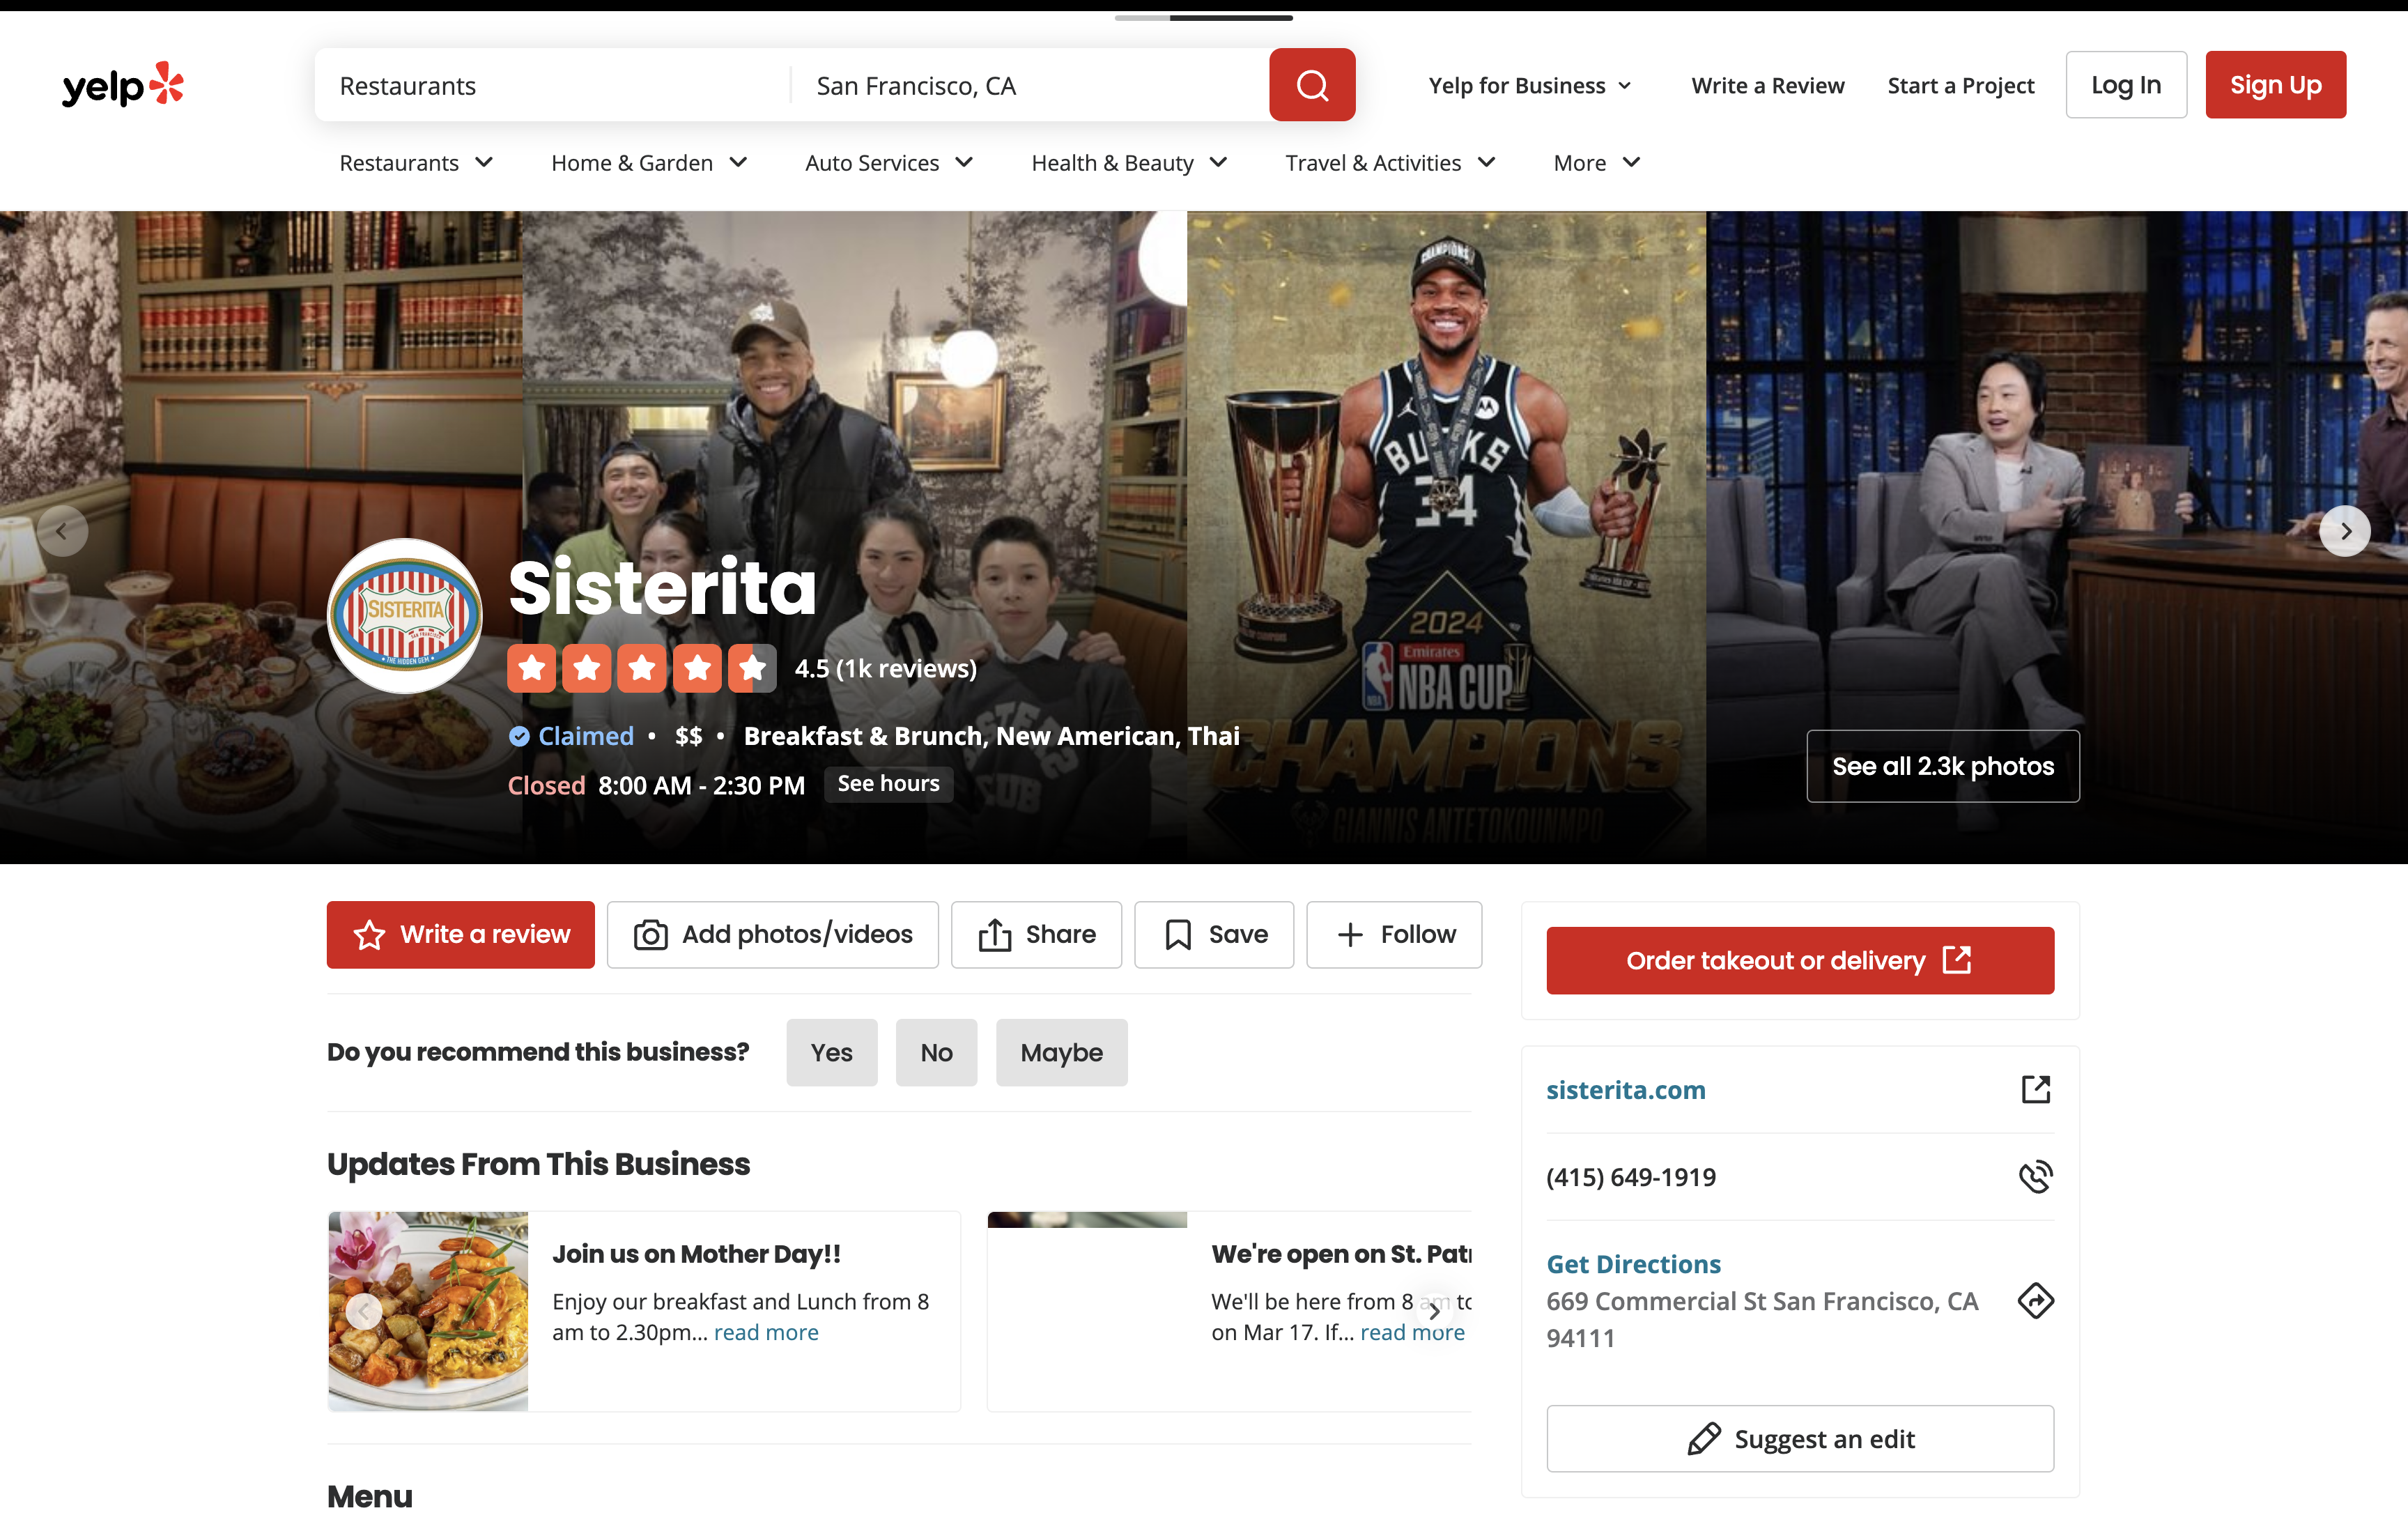
\includegraphics[width=0.9\linewidth]{yelp/restaurant view.png}
  \caption{Yelp Review Area — Insufficient feedback violating Nielsen H1 \& Norman Feedback}
  \label{fig:yelp-rest2}
\end{figure}

\textcolor{fixgreen}{\textbf{Tabla Fix:}} Reservation ends with a persistent confirmation screen (animated checkmark + booking code). Review flow ends with a ``Review submitted!'' success screen. Toast notifications use colour-coded states (green/amber/red). A progress bar (0\%→100\%) shows cinematic frame loading in real time. ``Open Now/Closed'' badges give live status on every card.

% ============================================================
\newpage
\section{Design Laws Applied in Tabla}
% ============================================================

\noindent The following subsections detail every HCI principle, law, and heuristic intentionally implemented in Tabla, with course-slide references.

% ── 3.1 ──────────────────────────────────────────────────────
\subsection{Fitts's Law \textnormal{\small[Lec~07, p.4--7]}}
$MT = a + b\log_2(2A/W)$. Target acquisition time decreases with larger width and shorter distance.
\textit{Applied:} 48\,px ``Find'' button adjacent to search input (zero extra movement); 44\,px full-width Reserve/Review/Dir buttons; centrally placed 44\,px Skip Intro; destructive ``clear'' as a small text link (intentionally hard to mis-tap).

% ── 3.2 ──────────────────────────────────────────────────────
\subsection{Hick's Law \textnormal{\small[Lec~07, p.8--9]}}
Decision time $\propto \log_2(n+1)$. \textit{Applied:} One primary hero action; five cuisine chips; four quick-filter options; six nav tabs ordered by usage frequency (Explore first, Sign In last).

% ── 3.3 ──────────────────────────────────────────────────────
\subsection{Miller's Law — 7$\pm$2 Rule \textnormal{\small[Lec~07, p.1]}}
STM holds $7\pm2$ chunks. \textit{Applied:} 6 card fields; $\leq$3 tag chips per card; 6 nav tabs; 5 shortcuts in overlay; time slots chunked into Lunch and Dinner blocks of 4--5 each.

% ── 3.4 ──────────────────────────────────────────────────────
\subsection{Jakob's Law \textnormal{\small[Lec~02, p.9; Lec~08, p.7--8]}}
Users prefer sites that match their existing mental models. \textit{Applied:} Logo at far-left sticky nav; heart for favourites; star + price symbol rating; three-step reservation mirroring Booking.com / OpenTable.

% ── 3.5 ──────────────────────────────────────────────────────
\subsection{Gestalt Principles}
\textbf{Proximity} (Lec~05): card actions grouped at card-bottom; chips in a single row. \textbf{Similarity}: all primary buttons share dark-oval style; all chips share rounded-pill shape. \textbf{Figure-Ground}: high-contrast wordmark over semi-transparent cinematic overlay. \textbf{Closure}: card images at consistent 220\,px height — no bottom crop ambiguity. \textbf{Continuity}: filter strip implies left-to-right scan from ``All'' to ``Nearby''. \textbf{Common Region}: each card is a rounded-rect with drop shadow forming one logical unit; modals use blurred overlay separating them from the page.

% ── 3.6 ──────────────────────────────────────────────────────
\subsection{Progressive Disclosure \textnormal{\small[Lec~06, p.4; Lec~08]}}
Show only essential information; reveal advanced options on demand. \textit{Applied:} ``More Filters~$\downarrow$'' hides dietary/ambiance/distance controls; reservation discloses one step at a time; review uses a three-step wizard; Cuisines tab reveals filtered list only after clicking a category.

% ── 3.7 ──────────────────────────────────────────────────────
\subsection{Feedback Principle \& Visibility of System Status \textnormal{\small[Lec~03, p.6,~9]}}
System must always inform users via appropriate feedback. \textit{Applied:} Real-time progress bar during cinematic preload; ``Scroll Down'' animated indicator; colour-coded toast notifications (green/amber/red); ``Open Now/Closed'' badge on every card; ARIA label toggles on heart icon.

% ── 3.8 ──────────────────────────────────────────────────────
\subsection{Tesler's Law — Conservation of Complexity \textnormal{\small[Lec~08, p.9--10]}}
Irreducible complexity must be absorbed by the system, not pushed to the user. \textit{Applied:} Reservation modal handles table-availability computation, date validation (\texttt{min = today}), and booking-code generation internally — user provides only 3 inputs.

% ── 3.9 ──────────────────────────────────────────────────────
\subsection{Doherty Threshold — 400\,ms \textnormal{\small[Lec~08]}}
Productivity is maintained when system response is $<$400\,ms. \textit{Applied:} Skeleton loader appears at 0\,ms (\texttt{SKELETON\_DELAY\_MS = 600}); search results rendered within 400\,ms (\texttt{SEARCH\_SKELETON\_MS = 400}); filter changes re-render grid synchronously on each click.

% ── 3.10 ─────────────────────────────────────────────────────
\subsection{Aesthetic-Usability Effect}
Aesthetically pleasing designs are perceived as more usable. \textit{Applied:} Cinematic frame-scroll intro; Playfair Display + Inter typography; gold accent \texttt{\#C9A96E}; 8\,px grid; card hover shadows; 800\,ms opacity transitions; animated confirmation checkmark.

% ── 3.11 ─────────────────────────────────────────────────────
\subsection{Recognition over Recall \textnormal{\small[Lec~03, p.4,~7]}}
Users should recognise options rather than retrieve them from memory. \textit{Applied:} Cuisine emoji identifiers; ₹/₹₹/₹₹₹ price symbols; star ratings; keyboard shortcut overlay (press \texttt{?}); active tab underlined + bold.

% ── 3.12 ─────────────────────────────────────────────────────
\subsection{Peak-End Rule}
Experiences are judged by their most intense moment and ending. \textit{Applied:} \textit{Peak} — cinematic frame-by-frame intro creates memorable first impression. \textit{End} — reservation confirmation features animated green checkmark + booking code; review flow ends with ``Review submitted!'' success screen.

% ── 3.13 ─────────────────────────────────────────────────────
\subsection{Von Restorff Effect — Isolation Effect}
Items that stand out are remembered better. \textit{Applied:} ``OPEN NOW'' badge in vivid green (\texttt{\#4A7C59}); gold ``Reserve'' button distinct from outline ``Review'' and ``Dir''; amber deal percentage badges in bold 800-weight text.

% ── 3.14 ─────────────────────────────────────────────────────
\subsection{Error Prevention \& Recovery \textnormal{\small[Lec~03, Nielsen H5/H9]}}
Prevent errors; help users recover gracefully. \textit{Applied:} ``Next'' disabled until time slot selected; date \texttt{min = today}; inline email regex validation; sign-in error banner without page navigation; autosaved review drafts (Raskin's 1st Law — Lec~08, p.1--3).

% ── 3.15 ─────────────────────────────────────────────────────
\subsection{Consistency and Standards \textnormal{\small[Lec~03, Nielsen H4; Shneiderman R1]}}
All primary actions use dark-background, white-text, 8\,px-radius buttons. All modals share backdrop blur, border-radius, and close-button position. Toasts always appear bottom-right; section headers follow the same hero-gradient + h1 pattern.

% ── 3.16 ─────────────────────────────────────────────────────
\subsection{Occam's Razor / Simplicity \textnormal{\small[Lec~08, p.10]}}
The simplest sufficient design is preferred. \textit{Applied:} Hero contains only the site name, one tagline, one search bar. Skip Intro is a two-word label. Cards omit phone/address — accessible via ``Dir'' when intentionally sought.

% ── 3.17 ─────────────────────────────────────────────────────
\subsection{Pareto Principle \& Zipf's Law \textnormal{\small[Lec~07, p.12--14]}}
80\% of usage comes from 20\% of features; the most-used action should be cheapest to perform. \textit{Applied:} Search, Reserve, and Favourite occupy the most prominent positions and largest touch targets. Advanced filters and keyboard shortcuts are accessible but de-emphasised.

% ── 3.18 ─────────────────────────────────────────────────────
\subsection{Accessibility \& Inclusive Design \textnormal{\small[WCAG~AA]}}
ARIA roles (\texttt{banner}, \texttt{search}, \texttt{main}, \texttt{progressbar}) and \texttt{aria-label} on every control; colour contrast $\geq$4.5:1 (WCAG AA); all elements keyboard-focusable with \texttt{:focus-visible} ring; ``Skip to main content'' as first DOM element; Escape dismisses all modals.

% ── 3.19 — Shneiderman ───────────────────────────────────────
\subsection{Shneiderman's 8 Golden Rules \textnormal{\small[Lec~03, p.1--4]}}
\begin{tabularx}{\linewidth}{@{}lX@{}}
\toprule
\textbf{Rule} & \textbf{Tabla Implementation} \\
\midrule
Strive for consistency     & Uniform button styles, modal patterns, toast colours \\
Shortcuts for power users  & \texttt{?} opens overlay; \texttt{Cmd+K} focuses search \\
Informative feedback       & Toast notifications, progress bar, skeleton loaders \\
Design for closure         & Reservation \& review each end with success screen \\
Error prevention           & Disabled ``Next'' until slot selected; inline validation \\
Locus of control           & Skip Intro; clear filters anytime; obvious ✕ close \\
Reduce memory load         & Emoji, stars, ₹ symbols, always-visible tab labels \\
Reduce short-term memory   & 6 card fields, $\leq$5 chips, $\leq$6 nav tabs \\
\bottomrule
\end{tabularx}

% ── 3.20 — Raskin's Laws ─────────────────────────────────────
\subsection{Raskin's Laws \textnormal{\small[Lec~08, p.1--6]}}
\textbf{Law~1 (Data Safety):} Review modal autosaves draft text to prevent accidental loss.
\textbf{Law~2 (Efficiency):} Geolocation auto-fills the Near Me tab; cuisine pill click on the hero directly filters the grid.
\textbf{Law~3 (Humane UI):} Single locus of attention per screen — modals disable background scrolling.

% ── 3.21 — Scroll/Fold behaviour ─────────────────────────────
\subsection{Scroll \& Fold Behaviour \textnormal{\small[Lec~06, p.1--4]}}
80\% of user attention is above the fold. \textit{Applied:} Hero search bar and CTA are fully above the fold; the animated ``Scroll Down'' indicator (false-floor prevention, Lec~06, p.4) signals additional content. After skipping intro, \texttt{revealMainApp()} scrolls the hero to top (zero extra scroll, Fitts-consistent).

% ── 3.22 — Horizontal Attention ──────────────────────────────
\subsection{Horizontal Attention — Left Lean \textnormal{\small[Lec~05, p.3--5]}}
Users' primary attention skews left-centre. \textit{Applied:} Logo and search bar are placed left-centre; the restaurant card image (the highest-attention element) occupies the left portion; ``Open Now'' badge overlays the top-left of each card image.

% ============================================================
\newpage
\section{Implementation Architecture}
% ============================================================

\subsection{Technical Stack}
TypeScript + Vite SPA with zero external UI libraries. Key modules:
\texttt{main.ts} (cinematic scroll), \texttt{grid.ts} (card renderer + filter engine), \texttt{pages.ts} (SPA router), \texttt{reservation.ts} (booking modal), \texttt{integration.ts} (cross-module event bus), \texttt{nav-hero.ts}, \texttt{accessibility.ts}, \texttt{shortcuts.ts}, \texttt{toast.ts}, \texttt{review.ts} (draft autosave).

\subsection{Cinematic Scroll Mechanics}
Three scroll phases over a canvas element rendering individual frames (\texttt{seq1/0001.jpg}~→~\texttt{seq2/0120.jpg}): \textbf{PHASE\_SEQ1} (wordmark fade-in), \textbf{PHASE\_BLUR} (quote interlude), \textbf{PHASE\_SEQ2} (cities + Explore CTA). At progress $\geq1$ or Skip click, \texttt{revealMainApp()} executes an 800\,ms CSS opacity transition and scrolls to top.

\subsection{Information Architecture}
\begin{verbatim}
Tabla
├── Cinematic Intro (Seq1 → Blur → Seq2 → Main App)
└── Main App
    ├── Explore — Hero Search, Filter Bar, Restaurant Grid
    │              → Reserve Modal / Review Modal
    ├── Near Me — Geo-sorted list
    ├── Cuisines — Category grid → filtered list
    ├── Saved — Favourites (localStorage)
    ├── Deals — Discount cards with countdown timers
    └── Sign In / Profile
\end{verbatim}

% ============================================================
\newpage
\section{User Personas \& Task Analysis}
% ============================================================

\textbf{Persona 1 — Priya} (26, Urban Professional, Chennai): Uses Tabla 4--5$\times$/week for lunch planning. Values speed and open-status accuracy. iPhone, primarily Search + Near Me.

\textbf{Persona 2 — Anand} (34, Fine Dining Planner, Mumbai): Visits 1$\times$/week for special occasions. Values rating credibility, price tier, table reservation. MacBook Safari.

\textbf{Persona 3 — Meera} (22, Budget Traveller, Bangalore): Checks Deals tab first. Values discount transparency and countdown timers. Android Chrome.

\textbf{Primary Task — Find \& Reserve:} Land on intro → Skip/Explore → search → scan grid → Reserve → Date/Time/Guests → Contact → Confirmation code.

\textbf{Secondary Task — Browse by Cuisine:} Cuisines tab → select category → browse filtered list → Reserve or Save.

% ============================================================
\newpage
\section{Slide Reference Map \& Additional Principles}
% ============================================================

\noindent The table below maps every design law used in Tabla to its course-lecture source. Rows marked~$\star$ are \textbf{extra principles} integrated beyond core lecture content.

\begin{longtable}{@{}p{3.8cm}p{1.6cm}p{1.4cm}p{7.2cm}@{}}
\toprule
\textbf{Principle / Law} & \textbf{Lecture} & \textbf{Page(s)} & \textbf{Key Insight \& Tabla Application} \\
\midrule
\endhead
Usability — 5 E's         & Lec~01 & 7      & Easy, Efficient, Effective, Enjoyable, Easy-to-remember \\
Affordance                & Lec~01 & 12     & Objects signal permissible operations; buttons look tappable \\
Visibility                & Lec~01 & 12     & Controls map clearly to effects; tab labels always visible \\
Mental Models             & Lec~02 & 1--4   & User beliefs shape interaction; Tabla mirrors familiar apps \\
Jakob's Law               & Lec~02 & 9; Lec~08 p.7--8 & Heart, stars, ₹ symbols all from known conventions \\
Skeuomorphism             & Lec~02 & 9--10  & Familiar real-world metaphors; booking flow mirrors physical reservation \\
8 Golden Rules            & Lec~03 & 1--4   & Consistency, Feedback, Closure, Control, Error prevention \\
Nielsen 10 Heuristics     & Lec~03 & 6--8   & H1 Status, H4 Consistency, H5 Error Prev, H7 Flexibility, H8 Minimalist \\
Norman's Design Rules     & Lec~03 & 9--10  & Feedback, Constraints, Mapping, Consistency, Affordance \\
Usability Dimensions      & Lec~04 & 1--2   & Learnability, Efficiency, Memorability, Errors, Satisfaction \\
Horizontal Attention Left & Lec~05 & 3--5   & Logo \& search bar left-centre; card image left \\
Gestalt Principles        & Lec~05 & --     & Proximity, Similarity, Figure-Ground, Closure, Continuity, Common Region \\
Scrolling \& Fold         & Lec~06 & 1--4   & Hero above fold; animated scroll indicator (false-floor prevention) \\
False Floor Warning       & Lec~06 & 4      & ``Scroll Down'' indicator invites scrolling past intro \\
Miller's Law (7$\pm$2)   & Lec~07 & 1      & 6 card fields, $\leq$5 chips, $\leq$6 tabs \\
Primacy \& Recency        & Lec~07 & 2--3   & Explore first, Sign In last in nav \\
Fitts's Law               & Lec~07 & 4--7   & 44px targets, proximal placement, $MT = a+b\log_2(2A/W)$ \\
Hick's \& Hyman's Law     & Lec~07 & 8--9   & One hero action; progressive-disclosure for extras \\
Pareto Principle (80/20)  & Lec~07 & 12--13 & Search/Reserve/Favourite are the prominent 20\% \\
Zipf's Law / Least Effort & Lec~07 & 14     & Most frequent action cheapest to perform \\
Raskin's Law 1 (Safety)   & Lec~08 & 1--3   & Review draft autosaved; no accidental data loss \\
Raskin's Law 2 (Efficiency)& Lec~08 & 4--5  & Geolocation auto-fills Near Me; cuisine pill filters directly \\
Raskin's Law 3 (Humane)   & Lec~08 & 6      & Single locus of attention; modal disables background scroll \\
Jakob's Law (full)        & Lec~08 & 7--8   & Design to existing conventions \\
Tesler's Law              & Lec~08 & 9--10  & System absorbs booking computation; user gives 3 inputs \\
Occam's Razor             & Lec~08 & 10     & Hero: name + tagline + search only \\
\midrule
$\star$~Aesthetic-Usability Effect & Extra & --  & Cinematic intro, gold palette, transitions raise perceived quality \\
$\star$~Doherty Threshold ($<$400\,ms) & Extra & -- & Skeleton loaders at 0\,ms; results $\leq$400\,ms \\
$\star$~Peak-End Rule     & Extra & --     & Cinematic peak; animated confirmation end \\
$\star$~Von Restorff Effect & Extra & --   & Green Open badge, gold Reserve button stand out \\
$\star$~Progressive Disclosure & Extra & -- & ``More Filters'' drawer; step-by-step modals \\
$\star$~WCAG AA Accessibility & Extra & --  & ARIA roles, 4.5:1 contrast, focus rings, skip-link \\
$\star$~Recognition over Recall & Extra & -- & Emoji, ₹ symbols, shortcut overlay \\
\bottomrule
\end{longtable}

\subsection{Usability Testing Plan}
\textbf{Method:} Think-aloud protocol (one session per persona). \textbf{Tasks:} (1) Find an open South Indian restaurant in Chennai. (2) Reserve for 4 at Burma Burma tomorrow. (3) Claim a deal. (4) Sign in and locate saved restaurants. \textbf{Metrics:} Task completion rate ($>$90\%), time-on-task, error rate, SUS score ($>$80), NPS.

\begin{center}
\begin{tabular}{@{}lll@{}}
\toprule
\textbf{Metric} & \textbf{Target} & \textbf{Method} \\
\midrule
Search-to-result latency  & $\leq$400\,ms   & \texttt{performance.now()} profiling \\
First Contentful Paint    & $\leq$1.5\,s    & Lighthouse audit \\
Reservation completion    & $\geq$90\%      & Observation \\
SUS Score                 & $\geq$80        & SUS questionnaire \\
Accessibility (Lighthouse)& $\geq$95\%      & Automated audit \\
Font contrast ratio       & $\geq$4.5:1 AA  & WebAIM Contrast Checker \\
\bottomrule
\end{tabular}
\end{center}

\subsection{Limitations \& Future Work}
Mock restaurant data; demo sign-in (\texttt{tabla123}); ``Dir'' opens Google Maps (embedded map view planned); pseudo-random time slots (real availability API needed); full VoiceOver/NVDA audit pending; localisation (Tamil, Hindi) not yet implemented.

% ============================================================
\newpage
\section*{References}
\addcontentsline{toc}{section}{References}
% ============================================================
\begin{enumerate}[leftmargin=1.5em]
  \item B.~Sivaselvan, \textit{CS5015 HCI Lecture Slides 01--08}, IIITDM Kancheepuram, 2025--26.
  \item J.~Nielsen, \textit{10 Usability Heuristics}, Nielsen Norman Group, 1994. \url{https://www.nngroup.com/articles/ten-usability-heuristics/}
  \item B.~Shneiderman et al., \textit{Designing the User Interface}, 6th ed., Pearson, 2016.
  \item P.~Fitts, ``Information capacity of the human motor system,'' \textit{J.\ Exp.\ Psych.}, 47(6), 1954.
  \item G.~Miller, ``The magical number seven, plus or minus two,'' \textit{Psych.\ Review}, 63(2), 1956.
  \item W.~Hick, ``On the rate of gain of information,'' \textit{Q.\ J.\ Exp.\ Psych.}, 4(1), 1952.
  \item D.~Norman, \textit{The Design of Everyday Things}, Basic Books, 2013.
  \item J.~Yablonski, \textit{Laws of UX}, O'Reilly Media, 2020.
  \item Yelp Inc., \url{https://www.yelp.com} (accessed February 2026).
\end{enumerate}

\end{document}